\problemname{Subset sum}
Eva vill bygga ett torn för att ta foton på Sandsjön. Hon har $N$ klossar av olika höjd.
För varje möjlig delmängd klossar kommer hon stapla de på höjd och klättra till toppen av tornet
för att ta en bild. Hon märker dock att många av dessa bilder blir samma! Detta kanske inte är så konstigt eftersom hon alltid tar samma bild för samma tornhöjd. Hur många unika foton kommer hon ha tagit när hon är färdig? 

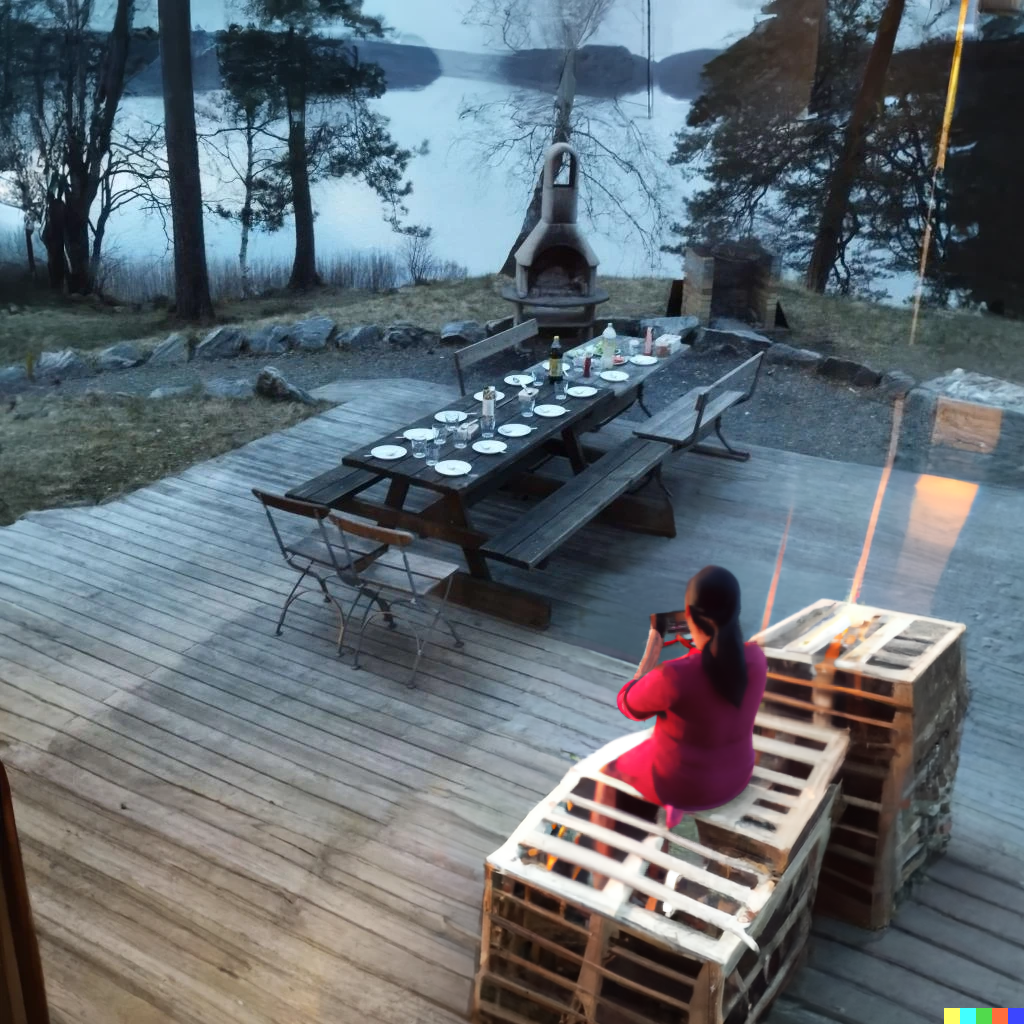
\includegraphics[width=10cm]{eva.png}

\section*{Indata}
Den första raden innehåller heltalet $N$ ($1 \leq N \leq 4000$), antalet klossar.
Därefter följer $N$ heltal $H_i$ ($H_i \leq 1000$), höjden på den $i$:te klossen.
\section*{Utdata}
Skriv ut ett heltal: antalet unika bilder som Eva tagit när hon är färdig.

\section*{Poängsättning}
Din lösning kommer att testas på en mängd testfallsgrupper.
För att få poäng för en grupp så måste du klara alla testfall i gruppen.

\noindent
\begin{tabular}{| l | l | p{12cm} |}
  \hline
  \textbf{Grupp} & \textbf{Poäng} & \textbf{Gränser} \\ \hline
  $1$    & $33$      & $N \leq 16$ \\ \hline
  $2$    & $33$      & $N \leq 100$ \\ \hline
  $3$    & $34$      & Inga ytterligare begräsningar. \\ \hline
\end{tabular}
